\documentclass{article}
\usepackage{fullpage,abstract,hyperref,graphicx,caption}
\usepackage{amsmath,amsfonts,amssymb,amsthm,program,float,multirow}

\makeatletter

\newfloat{algorithm}{thp}{lop}
\floatname{algorithm}{Algorithm}

\title{\vspace{-60pt}CS 6491 - Project 2 - Triangle Mesh}

\author{
\begin{tabular}{ll}
\multirow{3}{*}{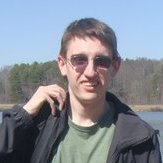
\includegraphics[scale=0.4]{chris.jpg}}\\&
Christopher Martin\\&\texttt{chris.martin@gatech.edu}\end{tabular}
~\\~\\~\\}

\newcommand\screenshot[1]{\includegraphics[scale=0.15]{#1}}
\newcommand{\argmin}{\operatornamewithlimits{argmin}}
\newcommand{\argmax}{\operatornamewithlimits{argmax}}
\def\p{\hspace{0pt}}

\begin{document}

\makeatletter
\twocolumn[
\begin{@twocolumnfalse}
\maketitle

\begin{abstract}

This project builds a Delaunay triangulation on a set of
randomly-generated vertices. The resulting triangle mesh is
used as the basis of a simple physics simulation in which
the mass at each vertex is accelerated by gravity and
a springlike force exerted by each triangle edge.
A click-and drag interface allows a user to break apart
triangles in a manner that somewhat resembles slicing through
a sheet of material.

\end{abstract}
\end{@twocolumnfalse}
]
\makeatother

\section{Delaunay triangulation}

Given the set of vertices $V$, we form
the mesh by calculating a Delaunay triangulation.
First we find a starting edge on the convex hull.
This edge is chosen as $(a,b)$ such that
\[ a = \argmin_{v \in V} v_y
\;\;\text{and}\;\;
b = \argmin_{v \in V} \textrm{angle}(v-a)
\;\text{.} \]
By repeating the process for determining $b$,
we simulate ``rolling'' a line around the outside
of the points, giving a calculation of the entire
convex hull.
These edges are not immediately added to the mesh,
but they are stored for later use.

\begin{figure}
\centering
\screenshot{init-debug}
\caption{Initial mesh configuration resulting
from Delaunay triangulation.}
\end{figure}

\begin{figure}
\centering
\screenshot{init}
\caption{A more aesthetically-designed rendering
of a denser triangle mesh.}
\end{figure}

We keep a work list of ``\textit{open}'' edges that
still need to be considered. While the \textit{open}
set is empty, the algorithm pops from it an edge $(a, b)$.
We form a triangle $(a,b,c)$ such that
\[ c = \argmin_{v \in V'} \text{bulge}((a,b), v) \]
where $V'$ consists of all vertices except $a$, $b$, and
any vertex that is part of a triangle with $a$ and $b$.
The new triangle is added to the mesh, and edges
$(a,c)$ and $(b,c)$ are each added to the \textit{open}
list if they are not on the convex hull.

Bulge$((a,b),c)$ is defined as the distance along a line
orthogonal to $(a,b)$, oriented toward $c$, from the
midpoint of $(a,b)$ to the circumscibing circle of
triangle $(a,b,c)$. Rather than calculate bulge directly,
we minimize a simpler computation
\begin{align*} \text{bulge}'((a,b),c) =&\;
\text{radius(a,b,c)}\\
&\times \text{side}((a,b), c) \\
&\times \text{side}((a,b), \text{cc}(a,b,c))
\end{align*}
where radius$(a,b,c)$ is the radius of the circumscribing
circle, cc$(a,b,c)$ is the triangle's circumcenter,
and side$((a,b),c)$ is either $1$ or $-1$ depending on
the side of line $(a,b)$ in which point $c$ resides.
This gives us that bulge$'$ correlates positively
with radius when the circumcenter is on the same side of
line $(a,b)$ as point $c$, and negatively when they
are on opposing sides.

Each triangle's vertices are sorted by angle around the
circumcenter to ensure that its corners'
\textit{next} and \textit{previous} values are consistent.
\textit{Swing} corners are determined using the simple
approach of searching for pairs of corners $i,j$ such that
$i${\p}.next{\p}.vertex $=$ $j${\p}.previous{\p}.vertex.
The corners are first grouped in a hash-multimap by vertex,
so the cost is quadratic only in the maximum vertex degree
rather than in the total number of corners.

\section{Physics}

At each time step of the physics simulation, the velocity
of each vertex $a$ is adjusted by multiple forces.
Gravity is a constant downward force.
For each adjacent vertex $b$, the spring force in the
direction of $b-a$ is proportional to the difference
between the edge's current length and its original length,
simulating Hooke's law.

Referring to the sum of these forces as $A$, we make
two changes to the current velocity $v$.
First, the acceleration is applied, reduced by some
inertial constant $I$.
\[ v \; \leftarrow \; \frac{1}{I}\left(v(I-1)+A\right) \]

Then damping is performed with a constant $D$,
introducing some friction and allowing motion to reach
a stopping point without oscillating indefinitely.
\[ v \; \leftarrow \; v \left( \frac{
  \max\left( 0, \Vert v \Vert - D \right)
}{\Vert v \Vert} \right) \]

\section{Cutting}

When the mouse is dragged between two points,
we first subdivide the range of motion into small
line segments to ensure that edge collisions can be
detected in the correct order.
Where the path crosses an edge,
we take the following actions:
\begin{enumerate}
\item Introduce a new vertex at the point where the
path crosses the edge (and make a note for future
reference of which vertex was just added).
\item Split the edge between the new vertex and the
previous most recently-added vertex by setting the
appropriate \textit{super-swing} values to \textit{true}.
\item If the split turned one of its vertices into a
non-manifold vertex, repair the mesh by creating a
duplicate of the vertex in the same position as the
original.
\end{enumerate}

\begin{figure}[h!]
\centering
\screenshot{cut}
\screenshot{cut-debug}
\caption{Two examples of cutting in progress.}
\end{figure}

\section{References}

\begin{itemize}
\item Intersection of a line and a circle\\
\texttt{http://mathworld.wolfram.com/\\Circle-LineIntersection.html}
\item Intersection of two lines\\
\texttt{http://en.wikipedia.org/wiki/\\Line-line\_intersection}
\end{itemize}

\end{document}

